%!TEX root = report.tex
\exercise{Highboost filtering}
\setcounter{subsection}{0}

Sometimes it is desirable to highlight high-frequency components in an image without eliminating the low-frequency components.
One way to do this is by using a technique called highboost filtering.
This technique works by first blurring the image, then subtracting the blurred image from the original image.
The result of this operation is called the \emph{mask}.
Finally, the highboost filtered image can be retrieved by adding the mask to the original image.

The entire highboost filter operation is nicely summed up in the following formula:
\[ g(x, y) = f(x, y) +  k(f(x, y) - w \star f(x, y)) \text{,} \]
where \(w\) is a smoothing filter, described below, and \(k\) a parameter that governs the magnitude of the filter.

As a result of the highboost filter, edges are sharper, while retaining most information about low-frequency components. 
\subsection{Implementation}
We have implemented the highboost filter in the function \texttt{IPhighboost}.
We have set the blur mask to the same mask as in \cite[Figure 3.32(a)]{gonzalez2002digital} which is also shown in Table~\ref{tbl:mask}.
\begin{table}[!htb]
  \begin{center}
    $\frac{1}{9}$
    \begin{tabular}{|c|c|c|}\hline
      1 & 1 & 1 \\ \hline
      1 & 1 & 1 \\ \hline
      1 & 1 & 1 \\ \hline
    \end{tabular}
    \caption{The Gaussian mask used for blurring}
    \label{tbl:mask}
  \end{center}
\end{table}

The following code implements the highboost filter operation\footnote{This function uses \texttt{IPfilter}, which is the same function as in the previous lab assignment. The source code for this is also included in the archive for this lab assignment.}:
\matlabexternal{IPhighboost.m}
When applying this function to \texttt{dipxetext.tif}, using multiple values for \(k\), the result in Figure~\ref{fig:dipxe} is retrieved.
The last image, with \(k=4.5\) is, in our opinion, the closest approximation to \cite[Figure 3.40(e)]{gonzalez2002digital}.

\begin{figure}[h]
 \centering
 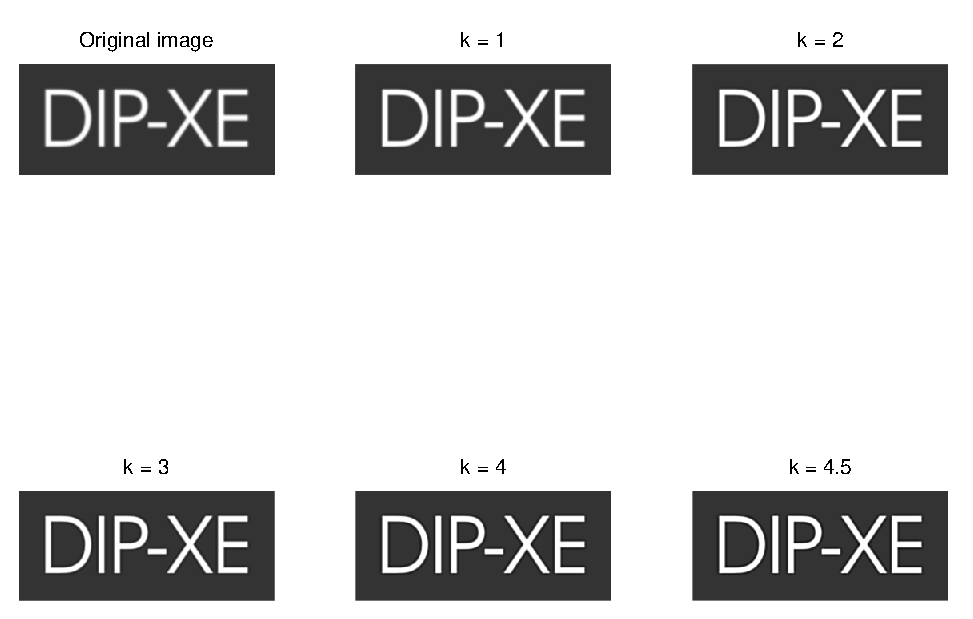
\includegraphics{dipxe.eps}
 \caption{Testing the highboost filter for several options of $k$. The image with $k = 4.5$, bottom-right, is the closest to image 3.40(e) in the book.}
 \label{fig:dipxe}
\end{figure}

\subsection{Negative values}
If an image \(f\) contains only positive values it is possible that the output image \(g\) contains negative values.
Consider the image depicted in Table~\ref{tbl:inImage}.
This image evidently contains only positive values.
However, if this image is processed using \texttt{IPhighboost} with \(k \geq 0.13\) the output image \(g\) will contain a negative value as table~\ref{tbl:outImage} illustrates.

A negative value occurs most notably when a pixel with a small value is surrounded by pixels with large values.
Consider a pixel in \(f\) at location \(( x_0, y_0 )\).
The value of that pixel after the highboost filter will be negative if:

\begin{equation} \label{zero_pixel}
  \begin{split}
    g(x_0, y_0) &< 0 \\
    f(x_0, y_0) +  k(f(x_0, y_0) - w \star f(x_0, y_0)) &< 0 \\
    k(f(x_0, y_0) - w \star f(x_0, y_0)) &< -f(x_0, y_0) \\
    k &< \frac{f(x_0, y_0)}{w \star f(x_0, y_0) - f(x_0, y_0)}
  \end{split}
\end{equation}

That is, the pixel \((x_0, y_0)\) will be zero at the critical value:
\[k_0 = \frac{f(x_0, y_0)}{w \star f(x_0, y_0) - f(x_0, y_0)}\]

When we compute the critical \(k\) for our example image in Table~\ref{tbl:inImage}, the value \(k_0 = 0.125\) is retrieved.

\begin{table}[h]
  \begin{minipage}[b]{.2\linewidth}
    \centering
    \begin{tabular}{|c|c|c|}\hline
    1 & 1 & 1 \\ \hline
    1 & 0.1 & 1 \\ \hline
    1 & 1 & 1 \\ \hline
    \end{tabular}
    \subcaption{Input image}
    \label{tbl:inImage}
  \end{minipage}
  \hfill
  \begin{minipage}[b]{.3\linewidth}
    \centering
    \begin{tabular}{|c|c|c|}\hline
      1.3278 & 1.2167 & 1.3278 \\ \hline
      1.2167 & -0.3000 & 1.2167 \\ \hline
      1.3278 & 1.2167 & 1.3278 \\ \hline
    \end{tabular}
    \subcaption{Output image (\(k=0.5\))}
    \label{tbl:outImage}
  \end{minipage}
  \hfill
  \begin{minipage}[b]{.4\linewidth}
    \centering
    \begin{tabular}{|c|c|c|}\hline
      1.0819 & 1.0542 & 1.0819 \\ \hline
      1.0542 & -0.0000 & 1.0542 \\ \hline
      1.0819 & 1.0542 & 1.0819 \\ \hline
    \end{tabular}
    \subcaption{Output image (\(k=k_0=0.125\))}
    \label{tbl:criticalImage}
  \end{minipage}
  \caption{The in- and output images for \texttt{IPhighboost}. Clearly, (b) shows that the regarded pixel is negative for \(k=0.5\). (c) shows that the regarded pixel is exactly zero for \(k=k_0\).}
  \hfill
\end{table}
\clearpage